\chapter{Introduction}




\section{Background}

In June 2009, the first Sunrise observatory \citep{SunriseI} was launched by NASA from Esrange Space Center, in Kiruna, Sweden, aboard a stratospheric balloon. Equipped with a 1-m aperture telescope, a multi-wavelength UV filter imager, SUFI \citep{SUFI} and IMaX \citep{IMaX}, a Fabry-Pérot-based spectropolarimeter, Sunrise was the most complex payload carried by a solar stratospheric balloon to date. The near absence of atmosphere at the altitude of the stratospheric balloons (approximately 36 km), allowed Sunrise the to achieve almost 24-hour continuous, seeing-free observations, along with the capability to measure the UV range, which cannot be observed from the ground. Aimed at studying the magnetic fields of the Sun and the dynamics of solar plasma convective flows, the mission was an outstanding success. It resulted in the publication of over a hundred peer-reviewed scientific articles in numerous high-impact journals, including Astronomy and Astrophysics (A\&A), The Astrophysical Journal (APJ), and Solar Physics, among others.

Following the success of its first flight, Sunrise embarked on a second journey  on June 13, 2013 \citep{SunriseII}. The primary objective of this second flight was to investigate Active Regions on the Sun, as it remained completely \textit{quiet} throughout the entirety of the first flight. Most of the original components from the first flight were reused for the second flight, with only minor refurbishments needed. This reuse was crucial to achieving a second flight within four years and at a relatively low cost. Despite the minimal modifications to the instrumentation aboard the observatory, the larger solar activity during this second flight yielded fresh perspectives and valuable data, ultimately securing the mission success, despite encountering some technical challenges.

Given the success of the first two flights, a third flight of the Sunrise mission was planned. For this third edition, the telescope was equipped with three post-focal instruments: SUSI, a UV spectrograph; SCIP, an infrared spectrograph; and TuMag, the evolution of the IMaX magnetograph. In addition to a new image correlator CWS and a new gondola and pointing system, provided by APL. Sunrise III was initially scheduled to fly during the summer of 2020 but was postponed to 2022.

The third launch of Sunrise plays a crucial role in this dissertation. This thesis, initiated in 2020, was centered on the development of the data reduction pipeline for the TuMag instrument, which was entirely developed by the Spanish space solar physics consortium. According to the original plan, the first half of the thesis was dedicated to the calibration of the instrument and the preparation of the data pipeline. This way, once the mission was launched, the second half of the thesis could focus on the correction and scientific analysis of the data produced during this third flight. However, this plan (and thus the scope of the thesis) encountered a setback on July 10, 2022, when the third flight of the Sunrise observatory had to be aborted just a few hours after the launch due to a mechanical failure during the ascent phase.

The observatory was recovered days later after a brief stay in the Scandinavian Alps. Both the telescope and the instruments were found to be in good condition, allowing for the recovery of the observatory and providing hope for a second attempt. However, the process of retrieving the instruments, disassembling, calibrating, and verifying their condition before relaunching the mission is lengthy, and it was not until the year 2024 that a second attempt became feasible.

In the absence of data produced by Sunrise to process, analyze, and exploit, the scientific work conducted within the framework of this thesis has been compelled to slightly shift its focus. Over these years, we have focused on delving deeper into image correction techniques for data obtained from Fabry-Pérot interferometers, such as TuMag and IMaX. Additionally, we have conducted several studies using data products from other instruments, such as the Polarimetric and Helioseismic Imager aboard Solar Orbiter (SO/PHI; \citealt{PHI}, \citealt{SO}) and the Helioseismic and Magnetic Imager of the Solar Dynamic Observatory (SDO/HMI; \citealt{hmi1}, \citealt{SDO}).

\begin{figure}
  \centering
  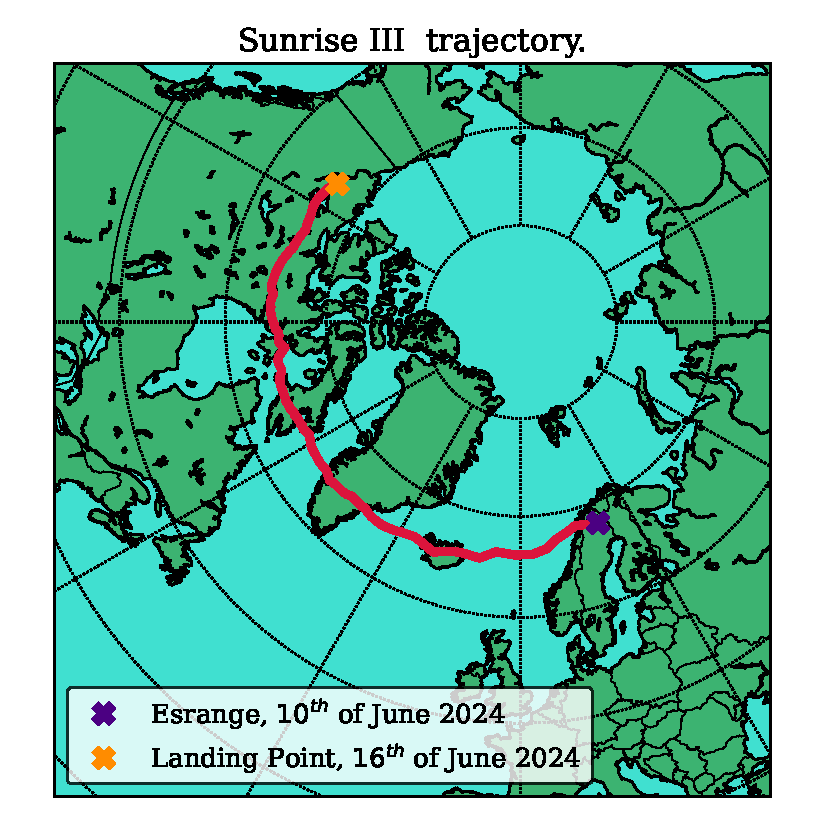
\includegraphics[width = \textwidth]{figures/Introduction/SunriseIII_trajectory.pdf}
  \caption[Sunrise III trajectory]{Sunrise III trajectory. Aqui poner tambien un foto de sunrise con el globo. } 
  \label{fig_intro: sunrise_trajectory}
\end{figure}

It wasn't until the 10$^{\text{th}}$ of July of 2024 that Sunrise III got its second chance to fly, and this time, the opportunity was not wasted. After a very succesful flight that lasted 6 days, the observatory landed in the northern region of Canada on the 16$^{\text{th}}$ of July. Figure \ref{fig_intro: sunrise_trajectory} shows the trajectory followed by our favourite solar observatory over these days. The recovery process started immediately after landing, and we were able to lay hands on the data for the first time on September 2024. 

\section{Motivation of our work}

In experimental sciences, there is a very strong relation between technological and scientific advances due to the simple fact that we cannot draw conclussions from what we cannot see. We believe it is important for experimental scientists, and more specifically, for observational astronomers, to know the limitations and capabilities of the techniques we employ and to understand the functioning of the instruments we use. 

This philosophy is one of the pillars of this thesis, which covers topics ranging from the design and calibration of scientific instruments to the exploitation of the data they produce. With this thesis, we aim to provide a broad, yet detailed, view of the various stages of a scientific mission, from its conception and objectives through its design and calibration, data reduction and preparation for scientific exploitation, and finally, the studies and conclusions derived from it.

In particular, I detail this process within the framework of solar physics through the development of TuMag, the magnetograph aboard Sunrise III. In the following chapters, I present the scientific objectives of the mission and attempt to link the design concepts with the scientific questions we aim to answer. I also present the work undertaken during the calibration and commissioning of TuMag, conducted in 2021, 2022, and 2024. I also address the challenges encountered in data correction due to the technical or instrumental limitations, a subject of ongoing debate within the community and of current relevance. Regarding this topic, I present the research carried out between the first and second flights of Sunrise III, which has resulted in the publication of two articles as the main author — one published in APJ and the other in A\&A — will also be detailed in this manuscript, as well as other studies that have not yet been published in any scientific journal. And finally, I also aim to offer a brief dip into the scientific explotation that can be carried out with the final data product. 

\section{Introduction}

Astronomy is one of the broadest fields of knowledge. It studies everything from the smallest astronomical objects, such as the small asteroids that inhabit our solar system, to the global structure and evolution of the universe, including the study of planetary systems, stars, black holes and the galaxies in which they are found. However, despite the diversity of disciplines—ranging from stellar astronomy, radio astronomy, and cosmology, to extragalactic astronomy, astrobiology, and solar physics—they all share a common tool for studying the cosmos: light. Since the very beginning of astronomy, the astronomer's work has been to learn how to modify and measure the properties of the photons that reach us in order to infer the characteristics of the observed object. Although recent advancements have provided astronomers with new lenses to \textit{see} the cosmos, like gravitational waves \citep{gravitational_waves} or neutrinos \citep{neutrinos}, among others, light remains as our main resource. Our understanding of the cosmos has always gone hand-in-hand with our ability to design and develop new and clever ways to disect the light, spanning from the first solar clocks, passing through Newton's first telescope to the modern-day spaceborne telescopes like the Hubble, James Webb or Solar Orbiter. 

Solar physics is no different from other astronomical disciplines in this regard. Our main tool to \textit{see} the Sun is through light. Contrary to what one may think, solar physicists are as photon-starved as any other astronomer. Even though our star is closer and (apparently) brighter than any other astronomical object, our requirements regarding resolution and sensitivity are so high that we are as dependent on extremely optimized instrumentation as any other discipline. Thus, the development of instrumentation employing state-of-the-art technology and techniques plays an important role in modern solar physics.

The interplay between technological innovation and our comprehension of the Sun drives the development of numerous new instruments and telescopes whose innovations open the window to new science. Notable examples include the Solar Orbiter mission \citep{SO}, a complex mission developed by the ESA and NASA and launched inb February 2020. Equipped with six remote-sensing and four in-situ instruments, Solar Orbiter is designed to study the Sun and the heliosphere from up close and from perspectives beyond the ecliptic, allowing for the monitorization of regions that cannot be observed from earth such as the poles. Another example is the \textit{Daniel K. Inouye} Solar Telescope \citep[DKIST;][]{DKIST}, a four meter aperture telescope at the Observatory of the Haleakal\=a Observatory in Hawaii, whose first operations commisioning phase took place in May 2020. With state-of-the-art adaptive optics and the largest aperture of any optical solar telescope worldwide, DKIST achieves an unparalleled spatial resolution, resolving solar features down to approximately 20 km. 

The same motivation lies behind the development of Sunrise and its three instruments.  The combination of the one-meter aperture of its telescope, the abscence of atmosphere, and the diversity of the scientific instruments makes Sunrise's observations unique. Designed to probe both the photosphere and the cromosphere, Sunrise provides a broad picture of the interaction of the phenomena ocurring at both layers with unprecedented level of detail.

Among the three scientific instruments aboard Sunrise is TuMag, a spectropolarimeter operating in the visible range of the optical spectrum, specifically designed to \textit{measure} plasma velocities and magnetic fields in the photosphere and chromosphere. The calibration and data reduction of TuMag represents the core of this thesis, with each topic addressed in its dedicated chapter. Given TuMag’s central role in this work, we begin the dissertation with a general overview of the properties and function of spectropolarimeters.


\section{A brief introduction to spectropolarimeters.}

As suggested by the name, spectropolarimeters are instruments designed to measure both the spectral and polarimetric properties of light. In other words, they assess the polarization state of light as a function of wavelength. Their use is widely extended in astrophysics, owing to the substantial amount of information that can be inferred about the light source from these properties.

There are two main types of spectropolarimeters, distinguished by their approach to spectroscopy: slit-based spectrographs and narrow-band tunable filtergraphs. The latter preserve spatial coherence by capturing two-dimensional images of the solar scene at the expense of sacrificing spectral resolution. Conversely, slit-based spectrographs provide excellent spectral resolution but the instantaneous two-dimmensional information is lost. 

Regardless of the method employed for spectroscopy, spectropolarimeters must be able to measure the polarization state of light, in other words, they must determine the Stokes parameters of the incident light. These four parameters, typically expressed as a pseudo-vector, $ \vec{I} = [I, Q, U, V] ^{T}$, were introduced by Stokes \citep{Stokes_vector} as a formalism to fully describe the polarization state of light. The first parameter, $I$, denotes the total intensity, while $Q$ and $U$ provide information on the intensity of linearly polarized light at 0º and 90º, respectively. Lastly, $V$ represents the intensity of circularly polarized light.


Outstanding polarimetric sensitivity and spectral resolution are rendered ineffective if the optical capabilities of the instrument are not up to par. The design of these instruments must achieve a signal-to-noise ratio that ensures the best posible polarimetric sensitivity for stokes Q, U and V. Additionally, it must provide the best spatial resolution that the telescope allows, all while maintaining high spectral resolution and minimizing observation time. Consequently, instrument design requires a careful balance among these three properties: spectral, optical, and polarimetric capabilities.

\textcolor{red}{In the following sections, we will examine each of these aspects in greater detail, with a particular emphasis on filtergraphs. Tunable filtergraphs play a significant role in this thesis, as the primary blocks of scientific work presented herein have been conducted for TuMag, a tunable magnetograph, as well as etalon-based instruments in general. Consequently, our description will be tailored to these types of instruments. It is important to note that much of the information provided will be generic and applicable also to slit-based spectrometry; however, certain specific behaviors will be unique to filtergraphs. }
Cambiar por simplemente especificar lo que se va a comentar. 

\subsection{Imaging and optical quality of Fabry-Pérot-based spectropolarimeters.\label{sec: intro-imaging}}

Filtergraphs are, first and foremost, imagers. The high-resolution imaging that filtergraph instruments are capable of is one of the pivotal reasons for their extended use. The ability to capture a two-dimensional scene of the solar surface makes them ideal for studying solar plasma structures, which require as large resolutions as posible. These instruments must be able to ensure an image quality and resolving power enough to measure these structures. For this reason, we will begin our description of the filtergraphs with a brief explanaiton of image formation and image quality assessment. 

Let us assume that the extended source we are observing has a instensity distribution in the image plane given by $O(\xi _ 0, \eta _ 0)$. Then, if we assume a linear optical system and incoherent illumination, the intensity distribution measured at a point $\xi, \eta$ of the image plane is given by : 

\begin{equation}
  I_ j\left(\xi, \eta ; \lambda_{s}\right)= \iint  O\left(\xi_0, \eta_0\right)  \mathcal{S}\left(\xi_0, \eta_0; \xi , \eta;\right)  \mathrm{d} \xi_{0} \mathrm{~d} \eta_{0},
  \label{eq_imaging: intensity_simple}
\end{equation}
where $\mathcal{S}\left(\xi_0, \eta_0; \xi , \eta;\right)$ represents the imaging response of the instrument, also referred to as the Point Spread Function (PSF). The PSF describes the normalized intensity distribution in the image plane when observing a point source, which, due to diffraction and inherent imperfections in any imaging system, cannot be imaged as an ideal point.

The PSF is crucial in the assessment of image quality and resolving power of an instrument since it defines how fine detail will be imaged into the detector. One particularly relevant metric for image quality assessment that can be derived from the PSF isthe optical transfer function (OTF), which is the Fourier transform of the PSF \citep{vargas_tesis}. 

\begin{equation}
  OTF(\nu) = \hat{\mathcal{S}}\left(\xi_0, \eta_0; \xi , \eta;\right),
\end{equation}
where the operator  $\ \hat{ }\ $  is the Fourier transform, and $\nu$ represents the frequency vector in the fourier domain.

The OTF describes how different spatial frequencies are transferred from the object to the image, thus characterizing the system's ability to resolve fine details. However, since imaging systems measure intensities, we are primarily concerned with how the intensity pattern of an object is transferred to the image plane. A key metric for quantifying this transfer is modulation, or contrast, which is defined as the ratio between the peaks and valleys of intensity at a given spatial frequency:

\begin{equation}
  M _ {\nu} = \frac{I_{max} ^{\nu} - I_{min} ^{\nu}}{I_{max} ^{\nu} + I_{min} ^{\nu}}.
\end{equation}

The function that encodes the dependency of the modulation with spatial frequencies is called the modulation transfer function (MTF), and is strictly related to the OTF as the ratio of the modulation of the object $MTF_{obj}$ and that of the image $MTF_{im}$. It can be computed from the magnitude of the OTF \citep{OTF}:

\begin{equation}
  MTF = \frac{MTF_{im}(\nu)}{MTF_{obj}(\nu)} = | OTF(\nu) |.
\end{equation}

From this definition, it is evident that a perfect optical system would have an $MTF=1$ at all spatial frequencies, meaning that all details are perfectly transferred from the object to the image. However, real optical systems exhibit a decrease in MTF as spatial frequency increases. In practice, the resolution of an optical system is often defined as the spatial frequency at which both the MTF and, consequently, the OTF reach zero \citep{wfes}. This threshold frequency marks the limit beyond which the system can no longer resolve finer details. 

Another key concept for assessing the imaging performance is the phase error or wavefront, $\phi$. The wavefront of an optical system is defined as the deviation in phase at any point within the image from that of an ideal spherical wavefront \citep{WFE_def}. Such deviations arise from various optical imperfections within the imaging system, and their impact on image quality depends on the specific nature of the aberration. For instance, imperfections in mirror shape or lens configuration can result in spherical aberrations, leading to a broadening of the PSF and a subsequent reduction in resolution. Other common aberrations include astigmatism, where the focal point varies along different axes, producing distorted images, and comatic aberrations (coma), which can occur due to misalignment of optical elements and manifest as tail-like distortions in the images of point sources.

It is common to see requirements or assessment of the optical quality of optical instrumentations in terms of the root mean square (rms) of the variance of the wavefront, $\Delta \phi (\xi, \eta)$, usually refered to as the wavefront error (rms WFE) or simply WFE:

\begin{equation}
  \textrm{WFE} = \sqrt{\frac{1}{A}\int _ {A} \Delta \phi  \left(\xi, \eta \right) ^2 \mathrm{d \xi}\mathrm{d \eta}},
\end{equation}
where $A$ is the area of the aperture. 

This value, essentially the standard deviation of the wavefront across the aperture, is closely tied to beam propagation quality. In fact, it can be demonstrated that the wavefront variance can be derived from the Strehl ratio, or viceversa, if only minor aberrations are present. The Strehl ratio is defined as the ratio of the peak intensity of a point source in an aberrated system to that of an ideal system operating at the diffraction limit. It is one of the most widely used metrics for assessing the optical quality of a system, ranging from 1, for a perfect, unaberrated system, to 0. For small aberrations, the Strehl ratio (SR) and WFE are related by the following expression \citep{WFE_def}: 

\begin{equation}
  \textrm{SR} \simeq \exp \left[ - \left(\frac{2\pi \textrm{WFE}}{\lambda}\right) ^2 \right].
\end{equation}

Although the Strehl ratio and rms WFE provide a concise measure of the optical quality of a system, the WFE contains additional information regarding imaging performance. Rather than relying solely on a single averaged value (such as the standard deviation), the wavefront can be represented as a two-dimensional map projected onto a plane normal to the light path, typically the image plane. To carry out such a representation analytically, it is essential to select an appropriate mathematical framework. Given the widespread use of circular apertures in telescopes, mirrors, lenses, and other optical components, it is advantageous to approach the problem using polar coordinates, $\rho$ and $\theta$, and in particular, to employ an orthonormal basis for the interpretability of the results. Among the multiple (infinite) sets of polynomials that fullfill these requirements, the Zernike polynimals \citep{Zernike} offer some distinct advantages. The Zernike polynomials are a sequence of polynomials that compose an orthonormal basis over a unit circle. Given an arbitrary wavefront, $W(\rho, \theta)$, the expansion in terms of the Zernike polynomials can be expressed as:
\begin{equation}
  W(\rho, \theta) = \sum_{n, m} C _n ^m Z _ n ^m(\rho, \theta),
\end{equation}
where $Z _n ^m$ are the Zernike polinomyals, $C_n ^m$ are the amplitues of the coeffiecients in the expansion and $n$ and $m$ are the radial order and angular frequency, repectively. The Zernike polinomyals can be obtained from:

\begin{equation}
  \left.
  \begin{array}{l}
  Z _ n ^m (\rho, \theta) = R _ n ^m (\rho) \cos (m\theta)\ , \ \text{for} \ m \geqslant 0 \ ,\\
  \\
  Z _ n ^{-m} (\rho, \theta) = R _ n ^m (\rho) \sin (m\theta) \ , \ \text{for}  \ m < 0 \ 
  \end{array}
  \right\}
\end{equation}
where $R _ n ^m (\rho)$ are the radial functions given by:
\begin{equation}
  R_n^m(\rho)=\sum_{l=0}^{(n-m) / 2} \frac{(-1)^l(n-l)!}{l!\left[\frac{1}{2}(n+m)-l\right]!\left[\frac{1}{2}(n-m)l-\right]!}\rho ^{n - 2l} \ .
\end{equation}

This representation of the wavefront is particularly valuable because each mode, defined by a specific pair of $n$ and $m$ values, corresponds to a distinct aberration in the wavefront, with the associated coefficient representing the contribution to the rms WFE for that specific aberration. Furthermore, the orthogonality of the Zernike basis ensures that adding additional terms to the expansion does not influence the values of previously calculated coefficients. In other words, the Zernike polynomial expansion enables the wavefront to be expressed as the sum of individual aberrations, providing a clear decomposition of the wavefront errors.

Figure~\ref{fig_intro: zernikes} presents an example of a simulated wavefront, including a two-dimensional cross-section and the individual Zernike components of the simulation. The simulation incorporates only the first ten Zernike polynomials, corresponding to polynomials with $n \leqslant 3$, which account for aberrations such as defocus, astigmatism, coma, and trefoil, among others. For a comprehensive overview of the Zernike expansion in wavefront characterization, we direct the reader to \citet{Zernike_guide}.

\begin{figure}
  \centering
  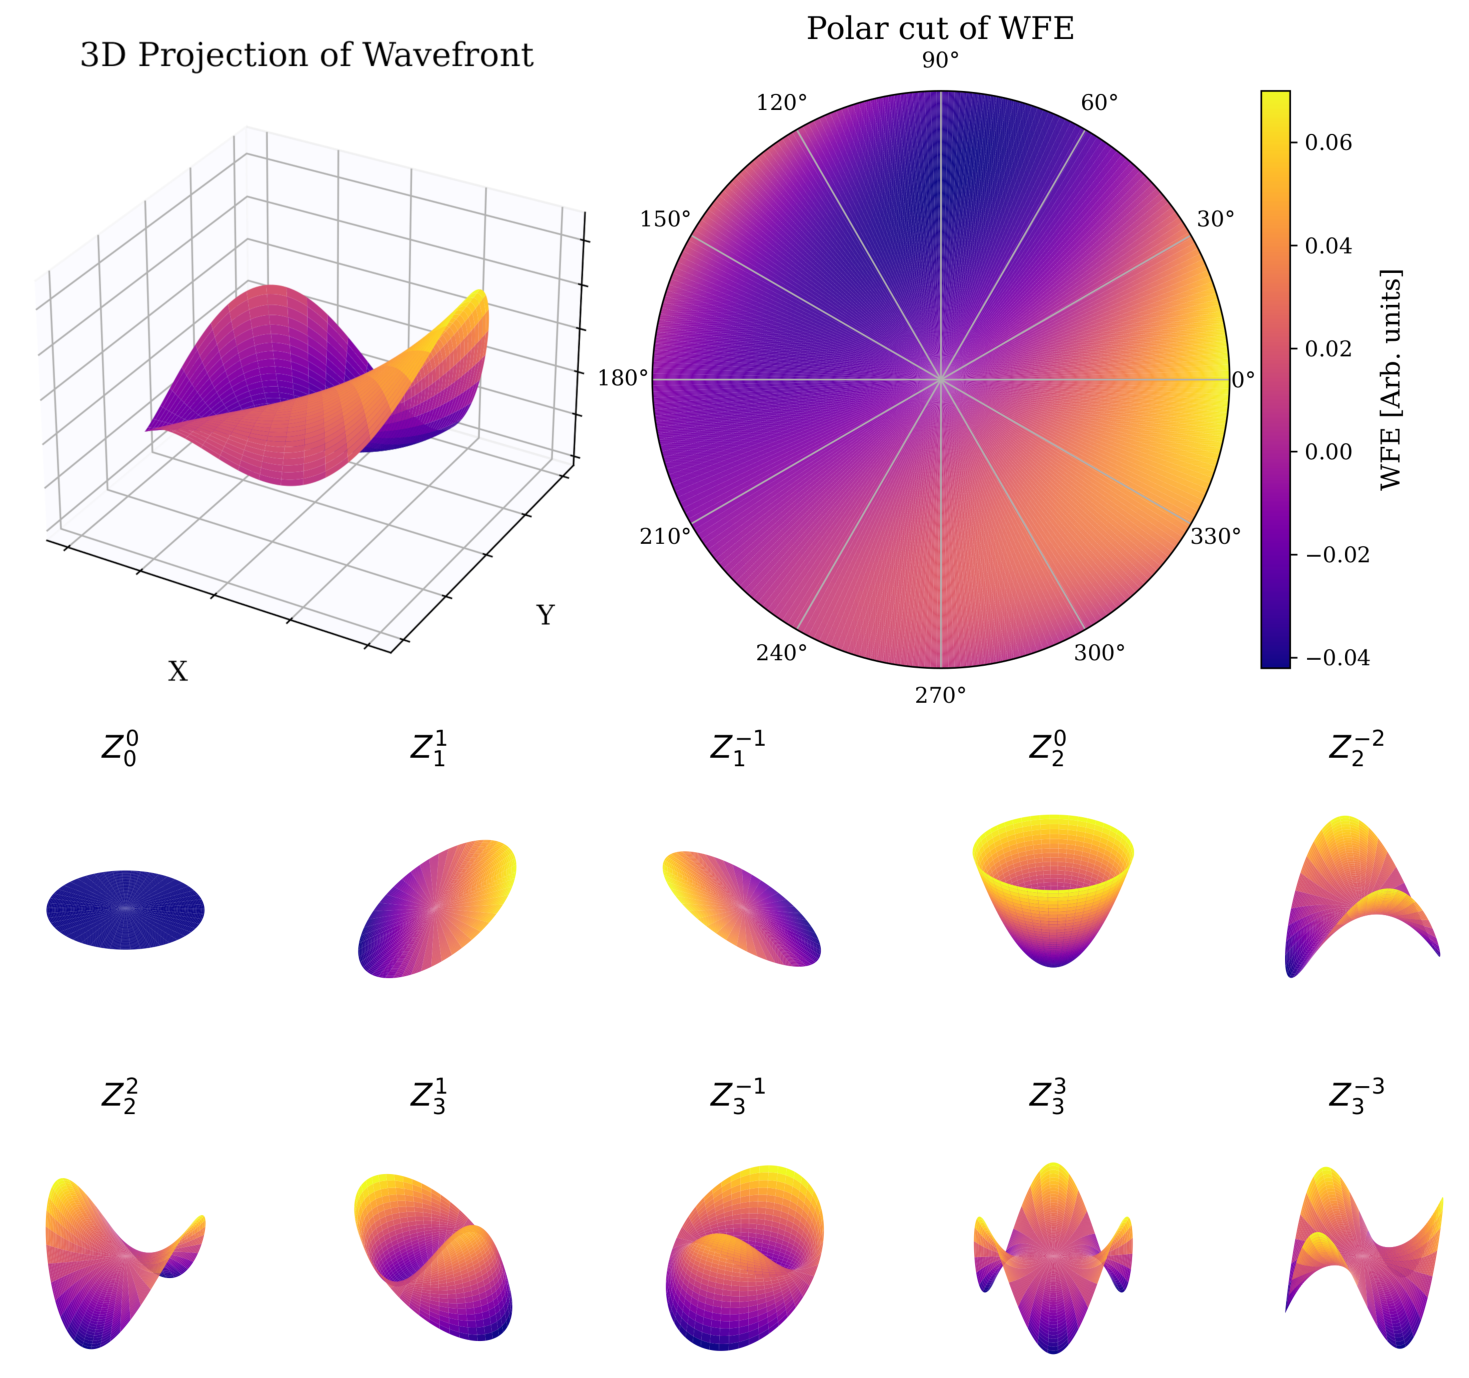
\includegraphics[width = \textwidth]{figures/Introduction/zernikes_combined.pdf}
  \caption[Zernike representation of wavefront error.]{Simulation of a wavefornt employing all zernikes with $n \leqslant 3$. The top left panel shows the 3-dimensional representation of the wavefront and the top right panel shows a cut in a plane normal to the direction of travel. The bottom two rows show the shape of the individual zernike polymials included in the simulation.} 
  \label{fig_intro: zernikes}
\end{figure}

Although properties such as the PSF and WFE offer valuable insights into the instrument's performance, they can vary between calibration phases and actual operation, or when the instrument moves from an isolated setup to integration with the full system. Therefore, instruments must have built-in methods to measure these properties during operation to evaluate performance and correct any arising defects. The strategy employed depends on the specific characteristics of the instrument. Among the different techniques, the phase diversity method is one of the most extended strategies. 

The phase diversity algorithm \citep{PD_original} is a method to infer the aberrations present in an optical system by obtaining, at least, two simultaneous, or quasi-simutaneous, images of the same object where an additional and known aberration is introduced to one of the images.  

The algorithm works by minimizing a cost function that depends on the OTF of the system which can be parametrized by the Zernike expanison \citep{pd_cost}: 

\begin{equation}
  \mathcal{L} (C) = \sum _ {k} \frac{|\hat{I_1} (\nu ) \hat{S_2} (\nu , C) - \hat{I_2}(u) \hat{S_1}(\nu , C)| ^2}{|\hat{S_1}(\nu , C)| ^2 + |\hat{S_2}(\nu , C)| ^2} , 
\end{equation}
where k represents the pairs of aberrated (subindex 1) and unaberrated (subindex 2) images, I stands for the intensity distributions, and S for the system's OTF expressed in terms of a Zernike expansion with coeffiecients C. 

By finding the coefficients of the zernike expansion that minimize $\mathcal{L}$, we are able to characterize the wavefront and identify the aberrations present in the optical system. Thus, determining the OTF, and consequently the PSF.

Our interest in determining the wavefront and OTF is not only to evaluate the instrument's performance but also to enable image restoration by mitigating the aberrations introduced during the imaging process. The procedure for removing the effects of the aberrations consists on removing the influence of the PSF on the final intensity distribution. In other words, the goal is to \textit{deconvolve} the PSF from the image.

Coming back to equation \eqref{eq_imaging: intensity_simple}, we can simplify the integrals to a convolution operator assuming an spatial invariance of the PSF. In that case, the observed intensity can be expressed by:

\begin{equation}
  I(\xi, \eta) = O(\xi, \eta) * S(\xi, \eta) + N (\xi, \eta)
  \label{eq_imaging: conv} 
\end{equation}  
where we added a term accounting for the noise present in real measurements $N (\xi, \eta)$.

The treatment of the problem is easier in the Fourier domain, where the convolution operator becomes a product of the fourier transforms of the corresponding functions. Therefore, in the Fourier domain, eq. \ref{eq_imaging: conv} becomes: 

\begin{equation}
  \hat{I}(\nu ) = \hat{O}(\nu)\hat{S}(\nu)+\hat{N}(\nu).
\end{equation}
Since neither $\hat{O}(\nu)$ nor $\hat{N}(\nu)$ are known, it is not possible to analytically derive the object, even if the system's response is known. Therefore, statistical approaches must be employed to deconvolve PSF.

One such approach is the Wiener-Helstrom filter \citep{wiener-helstorm}, which proposes that the estimated object, $\tilde{O}$, can be computed as:
\begin{equation}
  \tilde{O}(\nu) =  \frac{\hat{S}^{*}(\nu) \hat{I}(\nu)}{| \hat{S}(\nu)| ^2 + P_N (\nu) / P_O (\nu)},
  \label{eq_imaging: Wiener-Helstorm}
\end{equation} 
where the term $P_N(\nu) / P_O(\nu)$ represents the ratio between the power spectral densities of the noise and the object. Although this factor is unknown, it can be estimated based on the expected S/N in the data.

\subsection{Spectroscopy}

Among the tunable filtergraphs, Fabry-Pérot Interferometers (FPIs), also known as etalons (used interchangeably), represent one of the most prevalent forms of narrow-band tunable spectrographs. Composed by a resonant optical cavity formed by two distinct optical media, these devices allow only the passage of light with wavelengths corresponding to constructive interference within the cavity. 

The transmission profile of an etalon, being produced by an interference phenomenon, is characterized by a series of narrow and periodic transmission peaks. The wavelengths at which this resonance peaks are located, their width, and their separation are determined solely by the physical properties of the etalon. In fact, it is not difficult to demonstrate \citep{franI} that a resonant cavity produces a periodic transmission profile, with maxima occurring at a wavelength $\lambda$ such that:

\begin{equation}
\lambda = \frac{2nd\cos \theta}{m}\ ,
\label{eq_ch2: order_sorting}
\end{equation}
where $n$ is the refractive index of the medium inside the cavity, $d$ is the distance between the mirrors, $\theta$ is the angle of incidence of the incoming light ray and m is the interferential order ($m \in \mathbb{Z} $). 

With Eq.~\eqref{eq_ch2: order_sorting} in mind, it is clear that an etalon allows for tuning the wavelengths of the transmission peaks by either changing the distance between the mirrors or by altering the refractive index. Although changing the angle of incidence also results in a wavelength shift, it introduces additional modifications into the profile, in addition to a spectral shift. Consequently, the angle is not used for wavelength tuning.

To isolate a single wavelength, or a narrow band surrounding it, it is necesarry to employ the specific values of $n$ or $d$ that result in a tranmsision peak ocurring at that wavelength, often referred to as the main order, and block the rest of interferencial orders, known as secondary orders. This is typically achieved by using a pre-filter with a small bandwidth that only allows light with wavelengths near the desired measurement region to pass through. 

\begin{figure}
  \centering
  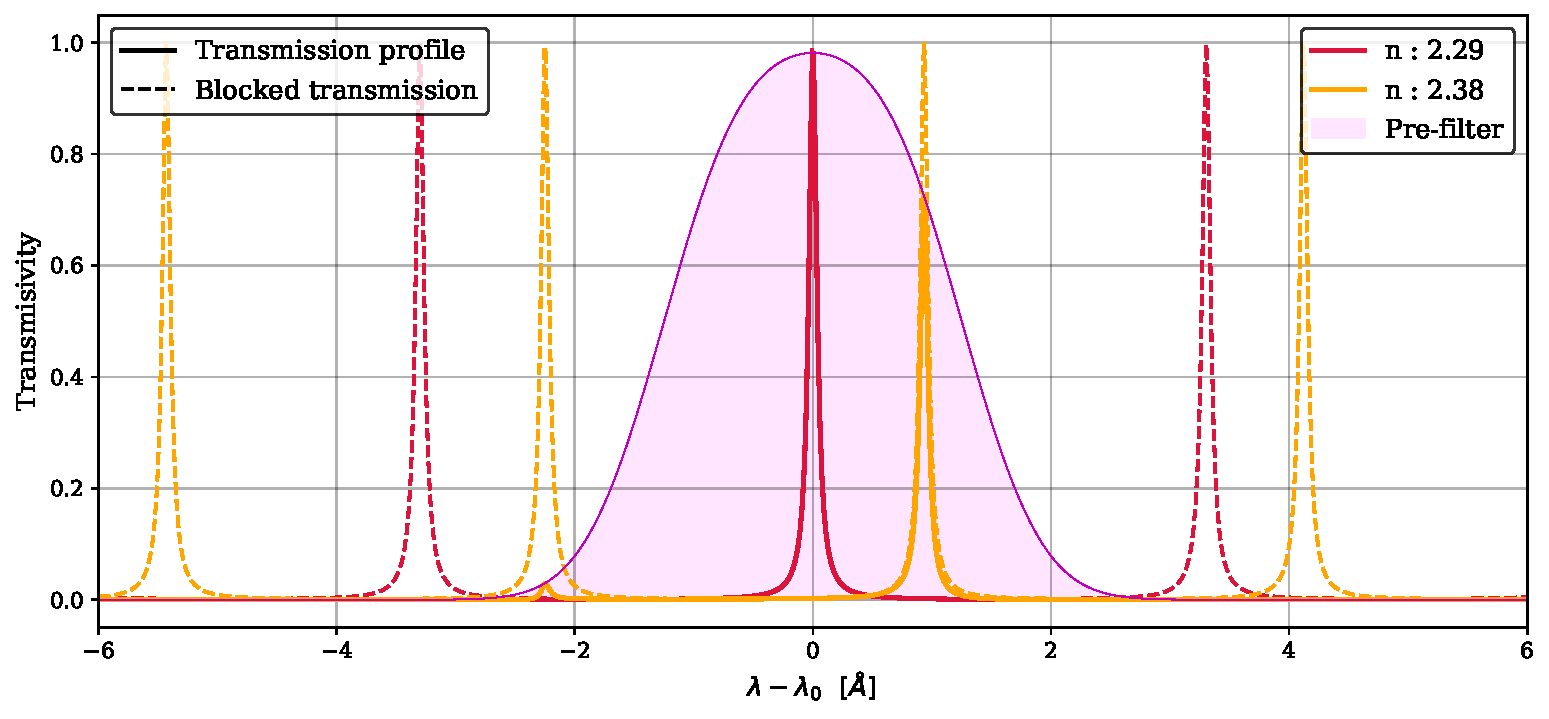
\includegraphics[width = \textwidth]{figures/Introduction_to_spectropolarimeters/Etalon_and_prefilter_example.pdf}
  \caption[Etalon's transmission profiles and prefilter.]{Transmission profiles of the same etalon with varying refractive indices (n). The dashed lines represent the original transmission profile, while the solid lines indicate the portion of the transmission profile that passes through the order-sorting pre-filter (shaded purple area).} 
  \label{fig_ch2: etalon_example}
\end{figure}

Figure \ref{fig_ch2: etalon_example} shows a simulation of the spectral behavior of this optical setup. The order-sorting pre-filter is shown with a shaded purple area and the unaltered transmission profile of the etalon is shown in dahsed lines for different values of the refractive index. In solid lines, the resulting transmission profile is shown, that is, the transmission allowed through both the pre-filter and etalon at the same time. 

\subsection{Polarimetry}

A polarimeter must be able to determine the Stokes components of the incoming light; however, these properties cannot be directly measured, as only the intensity of light is observed, not its intrinsic characteristics. Thus, polarimeters derive the Stokes parameters, rather than measure them. In order to do so, a series of multiple, simultaneous or quasi-simultaneous observations are taken, in which the polarization state of the incoming light is systematically altered. These different measurements, commonly referred to as modulations, are generated by inducing a known modification in the polarization. The Stokes parameters are then reconstructed by combining the information from all measurements through a process known as demodulation.

In order to understand how polarimeters derive the stokes components we need to briefly model how the different modulations are generated. Mathematically, the effect on polarization of a linear and finite system can be treated as a combination of linear transformations on the Stokes vector and, therefore, can be represented by a matrix in $\mathbb{R}^4$, known as the \textit{Mueller Matrix}. Let $\textbf{M}$ be the matrix that describes these transformations, then the polarization state that reaches the detector follows:

\begin{equation}
  \textbf{I}_{obs} = \textbf{M}\textbf{I}_{in},
  \label{eq_intro:modultaion_eqs}
\end{equation}
where $\textbf{I}_{in}$ and $\textbf{I}_{obs}$ are the Stokes vectors of the light that reaches the instrument, and the detector, respectively. However, since we only measure intensities, the actual quantity measured by our CCD is: 

\begin{equation}
  I_{obs} = m_{00}I_{in} + m_{01}Q_{in} + m_{02}U_{in} + m_{03}V_{in} \ \ ,
\end{equation}
where $m_{0i}$ is the i-th element of the first row of the Mueller Matrix. This means that the intensity we measure is a linear combination of the different polarization states of the incoming light. To determine the values of the individual parameters $I_{in}$, $Q_{in}$, $U_{in}$, and $V_{in}$, further independent measurements are necessary, which can be achieved by modifying the Mueller matrix. In particular, it is easy to see that four independent measurements are required in order to construct a system of equations that allows us to determine the full Stokes vector. This process is known as modulation, and the four independent measurements are the different modulations.

If we denote each of the modulations by $I _ j$ with $j \in \left\{ 1, 2, 3, 4\right\}$, we can construct the following system of equations:

\begin{equation}
  \begin{pmatrix}
  I _ 1 \\
  I _ 2 \\
  I _ 3 \\
  I _ 4
  \end{pmatrix} = 
  \underbrace{\begin{pmatrix} 
      m ^ 1 _ {01} & m ^ 1 _ {02} & m ^ 1 _ {03} & m ^ 1 _ {04} \\ 
      m ^ 2 _ {01} & m ^ 2 _ {02} & m ^ 2 _ {03} & m ^ 2 _ {04} \\
      m ^ 3 _ {01} & m ^ 3 _ {02} & m ^ 3 _ {03} & m ^ 3 _ {04} \\
      m ^ 4 _ {01} & m ^ 4 _ {02} & m ^ 4 _ {03} & m ^ 4 _ {04} 
  \end{pmatrix}}_ {\textbf{O}}
  \begin{pmatrix}
    I _ {in} \\
    U _ {in} \\
    Q _ {in} \\
    V _ {in}
    \end{pmatrix} \, 
    \label{eq_spectro_theory: stokes_linear_comb}
\end{equation}
where the superindex in $m ^j _{oi}$ denotes the values of the Mueller Matrix for each modulation, and $\textbf{O}$ is the so-called modulation matrix. Through straightforward algebra, it is easy to see that the stokes vector of the incoming light can be determined from the inverse of the modulation matrix, the demodulation matrix $\textbf{D}$: 

\begin{equation}
  \textbf{I}_{obs} = \textbf{M}\textbf{I}_{in}\longrightarrow \textbf{M} ^{-1} \textbf{I}_{obs} = \underbrace{ \textbf{M} ^{-1}\textbf{M}}_{\mathcal{1}}\textbf{I}_{in} \longrightarrow \textbf{D} \textbf{I}_{obs} = \textbf{I}_{in}
\end{equation}

Carefully determining $\textbf{O}$, and consequently $\textbf{D}$, during the instrument calibration process is crucial, as the accuracy of the determination of the Stokes components depends entirely upon it. It can be proven \citep{optimum_modulation} that the optimum modulation scheme—the values of $\textbf{D}$ that enable the Stokes vector to be computed with minimal uncertainty—satisfies the conditions:

\begin{equation}
  \varepsilon _ 1 \leqslant 1 \text{     , and     }, \sum _ {i = 2} ^4 \varepsilon _ i ^2 \leqslant 1,
  \label{eq_intro:optimum_efficiencies}
\end{equation}
where the polarimetric efficiencies for each stokes parameter (i = 1, 2, 3, 4), $\varepsilon _ i$, are defined as:
\begin{equation}
  \varepsilon _ i = \left( N_p \sum _ {j = 1} ^ {N_p} D _ {i, j} ^2\right) ^{-1/2},
  \label{eq_intro: polarimetric_efficiencies_definition}
\end{equation}
where $N_p$ is the number of independend modulations. 

When designing the modulation scheme for a given instrument, it is essential to satisfy the efficiency conditions given in Equation~\eqref{eq_intro:optimum_efficiencies} to ensure optimal polarimetric accuracy for all Stokes components. Furthermore, for equal sensitivities in the measurements of Stokes parameters Q, U, and V, the corresponding efficiencies should all be equal, with a value of $1/\sqrt{3}$. This is a very important result because polarimetric efficiencies are directly related to the smallest measurable polarimetric signals, the polarimetric sensitivity—essentially the inverse of the signal-to-noise ratio (SNR). This relation can be expressed as \citep{optimum_modulation}:
\begin{equation}
  \left( \frac{S}{N}\right)_i = \frac{\varepsilon _ i}{\varepsilon _ 1} \left(\frac{S}{N}\right)_1 \text{,    } i = 2, 3, 4 .
  \label{eq_intro: sn_and_efficiencies}
\end{equation}
From equations \eqref{eq_intro: sn_and_efficiencies} and \eqref{eq_intro:optimum_efficiencies} it is clear that the sensitivities for computing Stokes Q, U, and V will always be lower than that of Stokes I, as their corresponding efficiencies are smaller. To achieve an SNR of $10^3$ in Stokes measurements, which is the sensitivity required to detect weak polarization signals, an SNR of at least $ \left(S/N \right)_0 \gtrapprox 1700$ is necessary in the measurement of Stokes I for a quasi-optimal modulation scheme.

Spectropolarimeters ultimately combine measurements in polarization, spectral, and spatial (image) domains. Consequently, the final observed intensity depends on all three properties simultaneously. By integrating the spectral behavior of the etalon and pre-filter with the polatrimetric measurements, and taking into account the spatial dependence of these measurements, we can revisit equation \eqref{eq_imaging: intensity_simple} and rewrite it for FPI-based spectropolarimeters. In that case, the observed intensity for a modulation $j$ at any point of the focal plane $\eta, \xi$ when the etalon is tuned at a wavelength $\lambda _ s$ is determined by:
\begin{equation}
  I_ j\left(\xi, \eta ; \lambda_{s}\right)=g(\xi, \eta)\int_{0}^{\infty} T(\lambda) \iint  O _ j\left(\xi_0, \eta_0 ; \lambda\right)  \mathcal{S}\left(\xi_0, \eta_0; \xi , \eta; \lambda-\lambda_{s}\right)  \mathrm{d} \xi_{0} \mathrm{~d} \eta_{0}\mathrm{d} \lambda ,
  \label{eq_spectro: General_Intensity}
\end{equation}
where $T(\lambda)$ accounts for the presence of the order-sorting pre-filter, $S\left(\xi_0, \eta_0; \xi , \eta; \lambda-\lambda_{s}\right)$ accounts for the imaging response of the instrument when the etalon is tuned at the wavelength $\lambda_{s}$, $g(\xi, \eta)$ represents a spatial gain factor that accounts for any wavelength independent pixel-to-pixel intensity fluctuations ocurring in the focal plane, and $O _ j(\xi_0, \eta_ 0;\lambda)$ is the intensity distribution of the incoming light for a modulation j and is given by:
\begin{equation}
  O _ j(\xi_0, \eta_ 0;\lambda) = m_{00} ^jI_{in}(\xi_0, \eta_ 0;\lambda) + m_{01}^jQ_{in}(\xi_0, \eta_ 0;\lambda) + m_{02}^jU_{in}(\xi_0, \eta_ 0;\lambda) + m_{03}^jV_{in}(\xi_0, \eta_ 0;\lambda)
\end{equation}
 
\subsection{What do spectrpolarimeters tell us about the Sun?}

Spectropolarimeters are often referred to as magnetographs (\textit{e.g.}, TuMag), suggesting they measure magnetic fields directly. However, this is not entirely accurate. In astrophysics, the physical properties of the light source are inferred by correlating them with the observed properties of the light, rather than measuring them directly. By evaluating the polarization of sunlight at different wavelengths, spectropolarimeters enable us to infer the magnetic field and estimate plasma velocities on the solar surface. 

The simplest calculation we can carry out that provides us with physical quantities of the Sun is that of the line-of-sight (LOS) velocities. Given the spectral shift of a specific absorption or emission spectral line, $\Delta \lambda$, with respect to its rest position, $\lambda _ 0$ , the LOS velocities can be computed with the Doppler formula: 
\begin{equation}
  v_{\text{LOS}} = \frac{\Delta \lambda}{\lambda _ 0}c\ \ ,
  \label{eq_spectro: Doppler}
\end{equation}
where $c$ stands for the speed of light in vacuum. 

The polarization properties of light come into play when determining the magnetic fields. Due to Zeeman and Hanle effects, the polarity and spetcroscopy of spectral lines can be altered when formed in the presence of magnetic fields. Due to the Zeeman effect, the spectral lines widen or split into different polarized components when a strong magnetic field is present \citep{libro_JoseCarlos}, such as in the surroundings of sunspots and active regions. In the other hand, the Hanle effect is sensitive to weaker fields, and can be used to study, for example, the magnetic structure of solar prominences or turbulent fields in the solar photosphere \citep{hanle} where the fields are not strong enough to leave an imprint through the Zeeman effect.  

One simple strategy to employ polarization and spectral data to derive the magnetic fields is through the center-of-gravity method. According to \cite{center_of_gravity}, the LOS strength of the magnetic field can be obtained through:
\begin{equation}
  B_{\text{LOS}} = \frac{\lambda _ {+} - \lambda _ -}{2}\frac{4\pi m c}{eg_{L}\lambda_0 ^2}\ \ ,
  \label{eq_spectro: Blos-cog}
\end{equation}  
where $m$ and $e$ are the electron mass and charge respectively, $g_L$ stands for the Landé factor and $\lambda _ {+}$ and $\lambda _ {-}$ are the centroids of the right and left circularly polarized line components, respectively, and are computed by:
\begin{equation}
  \lambda _ {\pm} = \frac{\int \lambda \left[I_{\text{cont}} - (I \pm V)\right]d\lambda}{\int \left[I_{\text{cont}} - (I \pm V)\right]d\lambda} \ ,
  \label{eq_spectro: lambda_plus_minus}
\end{equation} 
where the subindex "$\text{cont}$" stands for the wavelength at the continuum. 

The vector magnetic field (\textit{i.e.}, strength, azimuth and inclination), and not only the LOS strength can also be derived. However, the derivation of these quantities has to be achieved through inversions of the radiative transfer equation (RTE). The applicability of the different methods to carry out this inversion is an extensive topic as there are some assumptions that can be applied in some cases but not in others, such as the weak-field or Milne-Eddington approximations, among others. For an extended discussion of this topic, we refer the interested reader to \cite{del2016inversion}.   